\section{Introdução}
\label{intro}

No desenvolvimento de software, há diversas variáveis, quer sejam de natureza ambiental ou técnica, que provavelmente impactarão desde a execução do processo de análise de requisitos até a implantação do software \cite{beckarticle1999}. Essa característica torna o processo de desenvolvimento pouco previsível e complexo, requerendo flexibilidade e personalização para ser capaz de responder às mudanças. 
Em consonância a esse movimento, órgãos da Administração Pública Federal (APF) também têm aderido a utilização de metodologias ágeis nos processos de desenvolvimento de software.

Recentemente, Tribunal de Contas da União publicou o Acórdão no 2314/2013 \cite{TCU:2013}
com práticas de contratação realizadas por instituições públicas federais, como por exemplo, Banco Central do Brasil (BACEN), Instituto do Patrimônio Histórico e Artístico Nacional (IPHAN), Instituto Nacional de Estudos e Pesquisas Educacionais Anísio Texeira (INEP), Tribunal Superior do Trabalho (TST) e Supremo Tribunal Federal (STF). 

Nestes órgãos, alguns casos de sucesso advém de processos de desenvolvimento interno e também por meio da transferência da execução tarefas executivas não ligadas com a função fim para iniciativa privada na prática conhecida comumente como terceirização de serviços que é apoiada pela legislação brasileira na Lei 8.666/1993 \cite{Lei8666:1993} que estabelece normas gerais sobre licitações e contratos administrativos; no Decreto-Lei 200/1967 que enunciou sobre a execução indireta de funções não finalísticas visando impedir o crescimento desmesurado da máquina administrativa e na Instrução Normativa nº 4 \cite{IN04:2010} que versa sobre o processo de Contratação de Soluções de Tecnologia da Informação pelos órgãos integrantes do Sistema de Administração dos Recursos de Informação e Informática do Poder Executivo Federal.

A Instrução Normativa nº 4 \cite{IN04:2010}, que é a norma mais recente, enuncia um conjunto e boas práticas e um modelo processo de contratações conforme visto na Figura \ref{processo}. 

\begin{figure}[h]
        \centering
        \label{processo}
            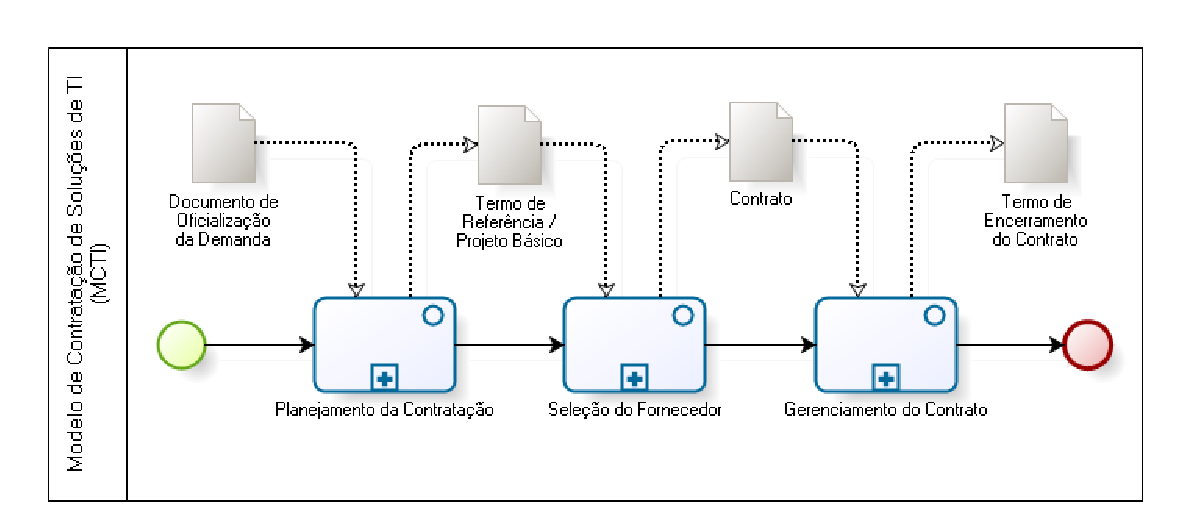
\includegraphics[scale=0.7]{figuras/MCTI.eps}
        \caption{Modelo de Processo de Contratações de Soluções de TI \cite{mcti}}
\end{figure}
\FloatBarrier	


A fase de Gerenciamento do Contrato visa acompanhar e garantir a adequada prestação do serviço e o fornecimento de bens que compõem a solução de TI, sendo que está disposto no art. 25, alínea b), que a avaliação da qualidade dos serviços realizados ou dos bens entregues e justificativas deve estar de acordo com os Critérios de Aceitação definidos em contrato, a cargo dos Fiscais Técnico e Requisitante do Contrato \cite{IN04:2010}.

Considerando o princípio ágil de valoração de produto sobre documentação abrangente, o foco na qualidade interna, e a necessidade das entidades da Administração Pública Federal do Poder Executivo, aferirem a qualidade do produto entregue por seus fornecedores de desenvolvimento de software, conforme previsto na alínea b) do art. 25 da \cite{IN04:2010}, o objetivo desta pesquisa foi:


\begin{tabular}{p{3.5cm}p{8cm}}
Analisar & \textbf{o código-fonte} \\
para o propósito  de & \textbf{aferir a qualidade interna} \\
com respeito à & \textbf{aceitação do produto} \\
do ponto de vista do & \textbf{fiscal técnico do contrato} \\
no contexto da & \textbf{contratação de desenvolvimento de software por parte da Administração Pública Federal} \\
\end{tabular}
